\documentclass[10pt,twocolumn]{article}
\usepackage[margin=0.75in]{geometry}
\usepackage{booktabs}
\usepackage{graphicx}
\usepackage[numbers]{natbib}
\usepackage{style/shisso}
\IfFontExistsTF{Noto Serif CJK JP}{\newfontfamily\jpfont{Noto Serif CJK JP}}{\newcommand\jpfont{}}
\usepackage{listings}\lstset{basicstyle=\ttfamily\scriptsize,breaklines=true,columns=fullflexible,keepspaces=true,frame=tb,framerule=0.3pt,aboveskip=4pt,belowskip=4pt,upquote=true}
\shissorepo{github.com/ravediamond/paper-register-reproducibility}
\input{shisso_commit}
\begin{document}
\title{What survives on a small team's rig: re-testing 21 robot-learning papers with cheap hardware and little data}
\author{Ravindu Somawansa\\Shisso Robotics\\\texttt{ravindu.somawansa@shissorobotics.com}\thanks{Every number with its source file: \texttt{github.com/ravediamond/paper-register-reproducibility}.}}
\date{}




\twocolumn[\vspace*{0.32in}\shissopanel{What survives on a small team's rig: re-testing 21 robot-learning papers with cheap hardware and little data}{Ravindu Somawansa\\[1pt]Shisso Robotics\\[1pt]\texttt{ravindu.somawansa@shissorobotics.com}}{Most robot-learning papers are tested in simulation or on rigs that cost more than \$20k; this is the case for 15 of the 21 papers we studied. We re-tested 37 of their claims on a rig of about €1,500, an SO-101 arm with a Jetson Orin NX. For each claim the bar was fixed before the test, and the cheapest baseline was run first on the same data. 12 claims hold and 18 fail. The failures take three forms: methods too slow for the edge GPU, judges that lose to the length of the episode, and learned latents that lose to the commanded joints. Many of these failures trace back to our small, short-task data as much as to the methods themselves. The code, the data and every number in the paper are public.}{\textbf{Code and rows:} \texttt{github.com/ravediamond/paper-register-reproducibility}\quad\textbf{Reproduce:} \texttt{make check}. Every number carries its source file and protocol commit.}\vspace{4pt}]
\section{Introduction}


Of the 21 papers in this study, 15 were shown in simulation or on a rig above \$20k, and only 2 on a rig under \$5k like ours. A small team that wants to use one of these methods has two options: trust the paper, or re-test the claim on its own hardware, which is slow and costly. The question we ask is simple: does a claim still hold for a small team, with cheap hardware, little data and short tasks?


To answer it, we took the claims one at a time and re-tested each on a single cheap rig. Adaptive chunking is a good example. The paper chooses the length of each action chunk from the entropy of several sampled chunks, so that the robot runs long chunks while moving between places and short ones at the grasp. To make one such decision the method samples 20 chunks, and on our Jetson Orin this took 4,751 ms, while our real-time budget is 298 ms. The claim fails on our rig. This does not mean it fails on the hardware it was shown on.


Over all the claims, 12 of 37 hold and 18 fail. Several of the failures are not near misses: the method loses to a baseline with no learning in it. Section 5 looks at these baselines, and Section 6 groups the failures into three classes. Section 7 then asks, for each failure, how much of it comes from the method and how much from our data and setup.


\section{Rig and data}


The rig is an SO-101 arm (five joints and a gripper) with a top camera and a wrist camera. Inference runs on a Jetson Orin NX 16 GB, and training runs on rented cloud GPUs. The priced parts cost €1,350 (2 small parts are not priced yet), and all the cloud GPU time came to \$42.30.


We used four sets of data. The first is our own teleoperated demonstrations (\texttt{so101\_bowls\_all\_trimmed}): 182 episodes and 61,462 frames at 30 fps, about 34 minutes in total, on two short tasks where one bowl is placed into another. We split them into 157 training and 25 validation episodes, and used them to train and test the world models and the VLA policies. The second is a set of rollouts of our trained policies on the arm (\texttt{so101-bowls-policy-rollouts}): 69 episodes, 44 successes and 25 failures, labelled by the operator. We used them for the failure monitors. The third is ArmnetBench \citep{arxiv260724481}, a public set of 2,099 labelled SO-101 rollouts from 7 policies, which we used for the reward models and judges. The last is 20 recorded episodes with 254 chunk boundaries, used for the chunking and latency tests.


This data has clear limits. All tasks are short, about 11 s per episode, and none needs several steps or memory, so we say nothing about long-horizon tasks. There is one task family, one arm and one room. The outcome labels come from a single operator and were not given blind.


\section{What we tested and how}


We chose papers from the parts of the stack our rig runs, and they fall into four kinds (Table 1). World models (7 papers) learn a latent from the camera to predict the next state or to plan; we test whether the latent predicts or plans better than a signal we get for free. Failure monitors and judges (7 papers) say whether an episode is failing or how far it has progressed; we test whether they catch failures better than a trivial signal. VLA policies (3 papers) follow an instruction on the arm; we test whether they succeed on our arm, over 10 trials judged by the operator. Chunking and edge inference (4 papers) concern how a policy's action chunks are produced and joined; we test whether the joins are smoother and how long a chunk takes on the Orin.


Every test follows two rules. First, the bar is written from the paper and its code only, before any result is seen, because a bar written after the result tends to drift toward it. Second, before the method itself, we run the cheapest baseline of its kind on the same data. The baseline is built from what we already have for free: the last frame, the joint values we send to the arm, the length of the episode, or the method with its main idea switched off. If the method loses to this baseline, its bar hardly matters. Each claim then gets one of four verdicts: it holds (the bar is met), it fails (the bar is missed), it is not proven (the test ran but cannot decide), or it is not tested yet.


A failure can also be our own fault, so where we could we ran a control. TurboVLA is the clearest case. We believed its architecture made our port of the policy ignore its instruction. We fixed the bar first: if swapping the task moved the output by $\geq$ 5°, the bug was in our port; if by $<$ 1°, the problem was the data. With the upstream trainer on our data, swapping the task moved the output by only 0.020°, while their released LIBERO checkpoint, run on our rig, moved it by 5.5°. The problem was our data, not their architecture. We withdrew the claim, and it is not counted in this paper.




\begin{table*}[t]\centering\footnotesize
\caption{The four kinds of papers, what we test in each, the cheapest baseline we build for it, and the verdicts.}
\begin{tabular}{p{3.0cm}p{1.1cm}p{4.0cm}p{5.2cm}p{3.6cm}}
\toprule
\shissohead kind of paper & papers & what we test & cheapest baseline & verdicts \\
\midrule
world models & 7 & predict the next state; rank or plan actions & copy-last (next state = current state); the commanded joints or the actions alone & 1 reproduce, 4 fail, 1 not proven, 1 not tested \\
failure monitors and judges & 7 & catch failures; track progress & episode length; the same model with shuffled actions & 7 fail \\
VLA policies & 3 & succeed on our arm & none cheaper: a success rate fixed before 10 trials & 3 reproduce \\
chunking and edge inference & 4 & smoother joins between chunks; time per chunk & the same policy without the trick; the real-time budget on the Orin & 2 fail, 2 not proven \\
\bottomrule
\end{tabular}
\end{table*}


\section{Results}


Figure 1 and Table 2 give the verdicts, and Table 1 breaks them down by kind of paper. Of the 37 claims, 12 hold, 18 fail, 3 are not proven and 4 are not tested yet. Counted by paper, 4 of the 21 reproduce, 13 fail, 3 are not proven and 1 is not tested. The pattern by kind is sharp: all 7 failure monitors and judges fail, while all 3 VLA policies reproduce. Section 7 shows that the first result is weaker evidence than it looks. The appendix gives every paper with its claim, its bar and our result.


\begin{figure*}[t]\centering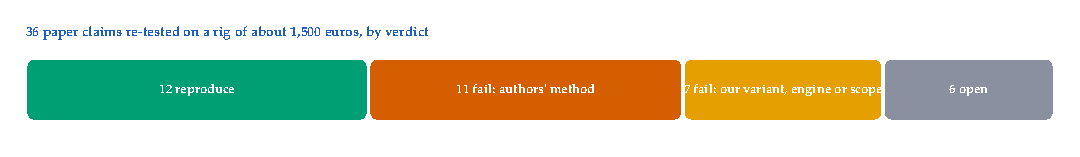
\includegraphics[width=\textwidth]{fig/verdicts.pdf}\caption{what survived when the papers left the lab: of the 37 paper claims, 12 reproduce and 18 fail; the failures fall into three classes: the clock, zero-shot judges against a trivial signal, and learned latents against the commanded joints.}\end{figure*}




\begin{table}[t]\centering\footnotesize
\setlength{\tabcolsep}{4pt}
\caption{Verdicts by paper and by claim.}
\begin{tabular}{lrr}
\toprule
\shissohead verdict & papers & claims \\
\midrule
reproduces & 4 & 12 \\
fails & 13 & 18 \\
not proven & 3 & 3 \\
not tested & 1 & 4 \\
\bottomrule
\end{tabular}
\end{table}


\section{The cheapest baseline}


The cheapest baseline is the signal we get for free on the same data as the method (Table 1). It needs no training and runs in minutes. We compared 11 paper claims with such a baseline (Table 3). The method clearly beat it in 4 cases, beat it by less than its bar in 2, and lost to it in 5.


The choice of baseline decides the verdict, even for a single model. LeWorldModel predicts the next latent far better than copy-last, with an error of 0.31 against 0.89, and that claim holds. Yet the same model ranks the chunk that was really executed worse than the actions alone do, 0.60 against 0.68--0.90, and that claim fails. Predicting well is not the same as planning well, and testing only one of the two would give the wrong picture.


The same baseline is also not equally strong on all data. On ArmnetBench, episode length beats the reward model (0.938 against 0.818), because there a failed episode tends to run until the time limit. On our own 88 rollouts, where failures do not run to the time limit, length is close to chance (0.521). What a judge must beat therefore depends on who stopped the episode, and the baseline has to be computed on one's own data.


Copy-last and the joints are strong partly because our task is short and simple: little moves apart from the arm, and the arm's state is already in the joints. On long tasks with many moving objects a learned latent has more to add, and we did not test that. Some papers report a cheap baseline themselves (shuffled actions for ReAP, a random pick for PACT-VLA, net joint displacement for HWM), and on our data those methods beat it too. Robometer reports no episode-length baseline. In practice, the baseline is the first thing to run: if the method loses to it, one can stop there, and only if it wins is the bar worth checking.




\begin{table*}[t]\centering\footnotesize
\caption{The paper claims we compared with a cheap baseline, on the same data.}
\begin{tabular}{p{2.6cm}p{4.2cm}p{3.0cm}p{2.4cm}p{4.4cm}}
\toprule
\shissohead method & baseline (what is measured) & method & baseline & outcome \\
\midrule
LeWorldModel & copy-last (latent error at 30 steps, lower is better) & 0.31 & 0.89 & beat \\
LeWorldModel & actions alone (executed chunk ranked first) & 0.60 & 0.68--0.90 & lost \\
DINO-WM & actions alone (executed chunk ranked first) & 0.61 & 0.68--0.90 & lost \\
RoboJEPA & copy-last (9-step latent error) & 11.8 \% below copy-last & -- & beat, under its bar of 15 \% \\
ContactGuard & the current latent (failure AUROC) & 0.70 & 0.82 & lost \\
ReAP & shuffled actions (failure AUROC) & 0.789 & 0.708 & beat \\
Robometer & episode length (failure AUROC, ArmnetBench) & 0.818 & 0.938 & lost \\
HWM & net joint displacement (cosine to the macro-action) & 0.608 & 0.551 & beat \\
Adaptive chunking & fixed chunk length (boundary jump, lower is better) & 0.973 & 0.940 & lost \\
PACT-VLA & a random pick (error of the executed window) & $-$0.27° against random & -- & beat \\
REMORA & per-frame readout (readout flips) & 0.70 $\times$ per-frame & -- & beat, under its bar of 0.5 $\times$ \\
\bottomrule
\end{tabular}
\end{table*}


\section{Three failure classes}


We see three classes in the failures. The first, class A, is the clock: the method does not fit the real-time budget of the edge GPU. Adaptive chunking needs 4,751 ms for one decision against a budget of 298 ms. It may well work on a faster GPU, and this class is the easiest to avoid, since a method can be timed on the target device before anything else is built.


Class B concerns judges, the models that say whether an episode succeeds, fails or progresses. A 4B reward model used zero-shot on ArmnetBench reaches an AUROC of 0.818, while episode length alone reaches 0.938.


Class C concerns learned latents, the vectors a world model computes from the camera. Our world model ranks the executed chunk first in 0.60 of anchors against a bar of 0.8, while a baseline using only the actions reaches 0.68--0.90. The commanded joints already hold the arm's state, so the latent has to add what the joints miss, such as where the objects are, and here it does not.


These classes are our proposal, based on the author's reading of the 18 failed claims, and a second reader would be needed to confirm them. They suggest an order for testing a paper on a cheap rig: time it on the device first, then compare it with the cheapest baseline, and only then look at its bar.


\section{Why they failed here: the method, our data, or our setup}


For each failure, Table 4 lists what on our side may explain it. Most failures have at least one such cause, so a failure here is a failure on this rig, with this data, and not a verdict on the method in general.


Our data is small and simple. We have 157 training episodes of one short task, about 11 s each, where the papers use hours of varied data; HWM, for instance, uses about 130 h against our 0.6 h. On a short task with one arm, the commanded joints already hold most of the state, which leaves little for a latent to add (class C). The task is also easy for our policy, since SmolVLA is at its ceiling on it, so there is little uncertainty for an entropy rule to read: the chunk length chosen by adaptive chunking sat at its minimum in 86 \% of decisions. For H-JEPA, our task lies outside the regime the paper targets, as there is no gap between slow and fast parts of the scene.


We also have too few failures. Our policies mostly succeed, and the main rollout set has only 8 failures in 50 episodes. A bar such as five failures caught out of eight is coarse, and a single episode can change the verdict (ReAP, VLA-Corrector, SURVEYOR).


In several cases our version of the method is not exactly theirs. For ContactGuard we used mixed policies and two cameras, where the paper uses one policy and three cameras. For FAIL-Detect and SAFE we used our world model's surprise as the score instead of their own scores. Our VLA-Corrector verifier works on pooled image statistics, not on their 54 features with the arm state. SURVEYOR's drafter is not released, REMORA's progress atoms are written by hand, and Robometer was only tested zero-shot because our fine-tuning run never trained.


Episode length is strong because of how the episodes end, not because judges are weak in general. On ArmnetBench a failed episode tends to run until the time limit, so length separates the outcomes (0.938); on our own 88 rollouts, where this is not the case, length is close to chance (0.521).


Our inference engine matters as well. vla.cpp samples sequentially and has no batching, so adaptive chunking pays for 20 full passes, while the paper's 106 ms was measured with batching on an A800. For PACT-VLA, the time of the check is projected rather than measured. Finally, several tests were offline only: planning ranked recorded chunks, and chunking measured smoothness on recorded episodes. None of these ran in closed loop on the arm.




\begin{table*}[t]\centering\footnotesize
\caption{Each fail or not-proven paper, what we measured, and what on our side may explain it.}
\begin{tabular}{p{2.8cm}p{1.8cm}p{5.6cm}p{6.6cm}}
\toprule
\shissohead failed paper & kind & our result & what may be on our side \\
\midrule
LeWorldModel & world model & planning rank 0.60, action-only 0.68--0.90 & one short task, 157 episodes, one seed; offline ranking only \\
DINO-WM & world model & planning rank 0.61, action-only 0.68--0.90 & same data as LeWorldModel; one training \\
RoboJEPA & world model & 11.8 \% below copy-last, bar 15 \% & near miss; the 1B model reached 15.8 \% on 30 clips only \\
H-JEPA & world model & progress ρ $-$0.73, bar $-$0.80; false stalls 52 \% & our task is outside the paper's regime \\
HWM & world model & not proven: high level worse at 2 s & 0.6 h of one task against their 130 h \\
ContactGuard & monitor & AUROC 0.70, current latent 0.82 & mixed policies and 2 cameras against one policy and 3 cameras \\
FAIL-Detect and SAFE & monitor & 22.7 \% of successes flagged at α 5 \% & our score, not theirs; 22 successes for calibration \\
ReAP & monitor & 3 of 8 failures caught & 8 failures only \\
VLA-Corrector & monitor & 2 of 8, AUROC 0.59 & our features, not their 54; 8 failures \\
Robometer & judge & AUROC 0.818, length 0.938 & zero-shot only; ArmnetBench failures run to the time limit (on our rollouts length is near chance) \\
SURVEYOR & monitor & threshold 1.249 against 0.20; 3 of 8 & their drafter not released; 8 failures \\
REMORA & monitor & readout flips 0.70 of the per-frame readout & hand-written progress atoms \\
Adaptive chunking & chunking & 4,751 ms per decision; length 2 in transport and at the grasp & sequential engine, no batching; task at ceiling for our policy \\
PACT-VLA & chunking & 37 ticks of delay against 8 & check time projected; sequential engine \\
Real-Time Chunking & chunking & not proven: 71--73 \% smoother, no arm run & offline smoothness only \\
Horizon $\times$ depth & chunking & not proven: 0.78, bar 0.70 & one policy, one task; arm test not run \\
\bottomrule
\end{tabular}
\end{table*}


\section{Limitations}


Our data covers one short task family, about 11 s per episode, with one arm, two cameras and about 34 minutes of demonstrations, so it says nothing about long-horizon tasks or varied scenes. There are few failures to test the monitors on, 8 in the main set of 50. Several methods are our own re-implementations rather than the authors' code end to end (Table 4), and the planning and chunking tests ran offline, never in closed loop on the arm. A single operator ran the arm and labelled the outcomes without being blind to them, and many tests use small samples and a single training seed. The VLA policies have no cheap baseline, only a success rate over 10 trials, which is a weaker test than the others. We chose the papers from the stack we run, so the rates describe these papers and not the field. Finally, a failure on our rig is not a failure on the authors' hardware, and our own mistakes are possible, as the TurboVLA case shows (Section 3).


\section{Related work}


Two works evaluate policies on the same arm: a real-world VLA benchmark with a taxonomy of failures and recoveries \citep{arxiv260608881}, and ArmnetBench, a fleet of SO-101 cells that evaluates policies at scale \citep{arxiv260724481}. In simulation, vla-eval runs VLAs across 14 benchmarks \citep{arxiv260313966}, and another benchmark studies the quality of demonstrations \citep{arxiv261018869}. These works rank policies. We instead take the claim a paper makes about its method and test it against a bar fixed in advance, on one cheap rig. The closest work is RoboSeed \citep{arxiv261040026}, which scores VLA and world-action models on five dimensions, including reproduction evidence and deployment affordability; its authors note that the score is not a probability that a result is correct. We give one yes or no per claim on one rig, with the data behind it.


\section{Conclusion}


We re-tested 37 claims from 21 robot-learning papers on a rig of about €1,500, with under \$50 of cloud GPU, and 12 of them held. Several methods lost to a baseline with no learning in it: copy-last, the commanded joints or the length of the episode. Our advice to anyone re-testing a paper on a cheap rig is to run the cheapest baseline first, on the same data, with the bar fixed before the test. Everything is public, and every number can be rebuilt from the repository. Authors who think a failure here is ours (Table 4) are welcome to tell us, and anyone with a cheap rig can run the same tests.


\bibliographystyle{plainnat}
\bibliography{refs}


\onecolumn
\appendix
\section*{Appendix: every paper}




\begin{table}[h!]\centering\scriptsize
\setlength{\tabcolsep}{3pt}\renewcommand{\arraystretch}{1.05}
\begin{tabular}{p{2.2cm}p{0.95cm}p{3.95cm}p{3.7cm}p{3.7cm}p{1.15cm}}
\toprule
\shissohead paper & their rig & claim tested & bar & our result & verdict \\
\midrule
\rowcolor{shissofail}LeWorldModel \citep{arxiv260319312} & sim & A small JEPA world model learns the arm's dynamics well enough to plan with it. & Dynamics: beat copy-last, every corruption $\geq$ 1.3 at K = 30. Planning: rank the executed chunk first among 8 in $\geq$ 0.8 of anchors. & dynamics 0.31 vs 0.89 copy-last (reproduces); planning top-1 0.60 vs 0.68--0.90 for an action-only baseline (fail) & fail \\
\rowcolor{shissofail}DINO-WM \citep{arxiv241104983} & sim & A predictor on frozen DINOv2 patches plans better than one on a learned latent. & G1b top-1 $\geq$ 0.8 at some target distance. & arm-pose R$^2$ 0.92 (vs 0.57 for W1); G1b top-1 0.55--0.61; no-model baseline 0.68--0.90 & fail \\
\rowcolor{shissofail}RoboJEPA \citep{arxiv261010515} & $>$\$20k & Pretrained RoboJEPA predicts our latents, uses the actions, and runs on the robot's computer. & 9-step L1 $\geq$ 15 \% below copy-last (300M) and $\geq$ 5 \% below shuffled actions; 2-view encoder $\leq$ 200 ms on the Orin. & 11.8 \% below copy-last (300M; 1B 15.8 \% on 30 clips); 9--10 \% below shuffled; encoder 526 ms on the Orin NX & fail \\
\rowcolor{shissofail}H-JEPA \citep{arxiv261006805} & sim & A slow second level makes latent distance track task progress. & Progress monotonicity Spearman ρ $\leq$ $-$0.80; false stalls $\leq$ 10 \%. & level-2 ρ $-$0.73; false stalls 52 \% & fail \\
D-JEPA \citep{arxiv260924749} & $<$\$5k & A decision-aligned ranking operator on a frozen world model picks better action chunks. & G1b regret $\leq$ 0.10 and $\leq$ the action-only baseline + 0.05. & regret 0.263 (W1 alone 0.263; action-only $-$0.007) & not tested \\
\rowcolor{shissofail}ContactGuard \citep{arxiv260813438} & \$5--20k & An event-anchored probe on imagined latents predicts grasp failure better than the current latent. & AUROC $\geq$ 0.85 and $\geq$ 0.05 above the current latent. & 0.70 imagined vs 0.82 current & fail \\
\rowcolor{shissofail}FAIL-Detect and SAFE \citep{arxiv250308558} \citep{arxiv250609937} & $>$\$20k & A conformal band on a learned failure score keeps false alarms at α while catching failures. & Successes flagged $\leq$ 1/20; failures flagged $\geq$ 50 \%. & 22.7 \% of successes flagged at α = 5 \%; 46 \% of failures caught & fail \\
\rowcolor{shissofail}ReAP \citep{arxiv261016309} & \$5--20k & A risk head on an action-conditioned latent warns before failures. & $\geq$ 5/8 failures caught at $\leq$ 1/20 false interventions; action-conditioned iff true $\geq$ shuffled + 0.05. & v1 AUROC 0.93 came from time and length; v2 0.789 vs 0.708 shuffled, 3/8 at 5/42 & fail \\
\rowcolor{shissofail}VLA-Corrector \citep{arxiv260906508} & sim & A verifier on observable history flags a failing rollout early enough to correct it. & $\geq$ 5/8 failures at $\leq$ 1/20 false interventions. & the paper's verifier family on our rollouts (a GRU on pooled RGB statistics and actions): 2/8 caught at 3/42 false interventions, AUROC 0.59; cosine drift of the W1 latent 0/8, AUROC 0.30 & fail \\
\rowcolor{shissofail}Robometer \citep{arxiv260302115} & $>$\$20k & A 4B reward model judges SO-101 rollouts zero-shot. & Pooled AUROC $\geq$ 0.85 and within-policy $\geq$ 0.8 on $\geq$ 5 of 7 policies. & pooled AUROC 0.818 on 2099 ArmnetBench rollouts; episode length alone 0.938 & fail \\
\rowcolor{shissopass}SmolVLA \citep{arxiv250601844} & $<$\$5k & A 450M VLA succeeds on an SO-101 task and can run on low-cost hardware. & 10-trial operator-judged gate (no numeric pass mark registered); chunk inference within the async budget (667 ms). & 9/10 on bowls; 974 ms in PyTorch, 238 ms with vla.cpp on the Orin NX & reproduces \\
\bottomrule
\end{tabular}
\caption{One row per paper with a claim of its own (internal model and test names kept). The rig price of €1,350 counts the parts with a stated price; 2 small parts are not priced yet. Read the verdict against the rig each paper was shown on.}
\end{table}
\begin{table}[h!]\centering\scriptsize
\setlength{\tabcolsep}{3pt}\renewcommand{\arraystretch}{1.05}
\begin{tabular}{p{2.2cm}p{0.95cm}p{3.95cm}p{3.7cm}p{3.7cm}p{1.15cm}}
\toprule
\shissohead paper & their rig & claim tested & bar & our result & verdict \\
\midrule
\rowcolor{shissopass}VLA-JEPA \citep{arxiv260210098} & sim & VLA-JEPA trains cheaply on SO-101 data and runs on the robot. & 10-trial operator-judged gate (no numeric pass mark registered); for reranking (H0): oracle / mean error $\leq$ ~0.7 and N = 8 $\leq$ 1.5$\times$ the latency. & 9/10 for ~\$9.7; 355 ms per chunk on the Orin NX; reranking no-go (0.76, 1.84$\times$) & reproduces \\
\rowcolor{shissopass}REKI \citep{arxiv261022178} & sim & Policies without memory oscillate between poses at a measurable rate. & $\geq$ 10 \% of failed episodes oscillate (their criterion). & 20.3 \% of all episodes, 24.0 \% of failures; REKI trained on my data: 19/20 + 19/20 on the arm, oscillates in 1/40 & reproduces \\
\rowcolor{shissoamber}Real-Time Chunking \citep{arxiv250607339} & unstated & Conditioning a new chunk on the executing one removes the jump at chunk boundaries. & Best gradient-free method cuts the median jump $\geq$ 50 \% against naive async, drift $\leq$ +10 \%, within 667 ms. & prefix overwrite cuts the jump 71--73 \% against naive async at +0.4 ms; tuned LeRobot identity mode is close & not proven \\
\rowcolor{shissoamber}HWM (hierarchical latent world models) \citep{arxiv260403208} & $>$\$20k & A high-level world model over learned macro-actions beats the low-level model beyond about 1 s (their Fig. 6 crossover). & Crossover in [1.0, 2.0] s; at 2 s high-level error $\leq$ 0.95 $\times$ low-level; learned macro-actions $\geq$ net joint displacement on cosine. & no crossover: W1 0.382 $\pm$ 0.005 $\rightarrow$ 0.563 $\pm$ 0.007, high level 0.769 $\pm$ 0.009 $\rightarrow$ 0.759 $\pm$ 0.009 (0.73--2 s); cosine 0.608 $\pm$ 0.007 vs 0.551 $\pm$ 0.006 & not proven \\
\rowcolor{shissopass}LeJEPA identifiability \citep{arxiv260526379} & sim & A SIGReg JEPA trained on goal-directed data recovers the true latent state only partially and unevenly. & W1's mean R$^2$ from latent to joints $<$ 0.80; anisotropy (max $-$ min per-joint R$^2$) $\geq$ 0.20; the higher-R$^2$ model has the higher G1b top-1. & W1 mean R$^2$ 0.565, anisotropy 0.639 (shoulder lift 0.91, wrist flex 0.27); frozen DINOv2-S 0.867 / 0.301 & reproduces \\
\rowcolor{shissofail}SURVEYOR & sim & A threshold on the imagined-vs-reached latent distance accepts good plans and rejects bad ones ($\tau$ = 0.20). & $\tau$ below the 10th percentile of non-equivalent pairs and $\leq$ 0.40; as a monitor $\geq$ 5/8 failures at $\leq$ 2/42; $\geq$ 0.05 AUROC over a shuffled drafter. & $\tau$ = 1.249 on W1 latents of 69 real rollouts; as a monitor 3/8 at 6/42 (S = 30), AUROC 0.756 vs shuffled 0.560 & fail \\
\rowcolor{shissofail}Adaptive Action Chunking (AAC) \citep{arxiv260404161} & $>$\$20k & Chunk length chosen from the entropy of N sampled chunks follows the task's phases (long in transport, short at the grasp), lowers the boundary jump, and costs little with batched sampling. & median h* in transport $\geq$ grasp window + 2; jump with AAC + overwrite $\leq$ fixed + overwrite at d = 8; an N = 20 decision $\leq$ 298 ms on the Orin. & h* 2 in transport and 2 at the grasp (86 \% of decisions at the floor); jump 0.973 vs 0.940; N = 20 decision 4,751 ms (sequential) on the Orin & fail \\
\rowcolor{shissofail}PACT-VLA \citep{arxiv261028019} & \$5--20k & Picking among N sampled chunks by their flow residual under the pre-commit observation fits what happens next better than a random or stale pick, with no added control-step delay. & PACT beats a random pick and the stale-observation residual at d = 8 (CIs $<$ 0); its delay on the Orin $\leq$ the naive delay; at that delay it still beats a single sample. & offline $-$0.27° vs random and vs the stale residual (both CIs $<$ 0); on the Orin 1,200 ms per cycle, 37 control ticks vs 8 & fail \\
\rowcolor{shissoamber}Horizon $\times$ depth (Euler steps vs execution horizon) \citep{arxiv261032102} & $>$\$20k & With long open-loop commitment, cutting a flow-matching VLA's Euler steps from 10 to 2 contracts the action cloud around an unchanged centroid, saves most of the inference time and avoids edge-GPU thermal throttling. & median R(2)/R(10) $\leq$ 0.70 with the centroid within 0.05 relative and 3°; N = 2 latency $\leq$ 0.85 $\times$ N = 10 on the Orin, N = 10 within 5 \% of 238 ms. & R(2)/R(10) 0.78 (CI 0.73--0.81), centroid 0.018 and 2.35°; 196.1 vs 237.5 ms per chunk (0.83, vision 151 ms); no throttling at N = 10 on the Orin, at MAXN\_SUPER or 25 W & not proven \\
\rowcolor{shissofail}REMORA \citep{arxiv261039125} & $>$\$20k & Reading a progress distribution out at the supported peak nearest the previous estimate steadies the estimate and lets it fall during real setbacks, with no worse detection of the stages. & Against per-frame argmax: premature not higher and missed $\leq$ +2 points (P1); flips halved, CI upper $\leq$ 0.7 (P2); a decrease inside $\geq$ 50 \% of the reversal windows with $\leq$ 20 \% false regressions (P3). & premature 0.22 vs 0.25, missed equal (P1 pass); flips 0.70 $\times$ argmax, CI 0.48--0.94 (P2 fail); setback recall 2/7, false 0.52 (P3 fail); MAE 0.184 vs median 0.218 & fail \\
\bottomrule
\end{tabular}
\par\medskip Table 5, continued.
\end{table}
\end{document}
